\section{Implementation and Experiments}

\subsection{Clause Reduction with $\IUIP$}
To evaluate $\IUIP$'s effectiveness as a clause reduction technique, we implement  $\IUIPPURE$ and $\IUIPMIN$  on top of \text{\MapleBase} \cite{}, the winner of SAT Race 2015 application track.  We than compare the performance of the baseline $\MapleBase$ with $\MapleIUIPPURE$ and $\MapleIUIMIN$ on the full set of benchmarks from SAT RACE 2019 main track.

The benchmark contains 400 instances divided into two groups of 200, new and old, representing historical instances and fresh instances in the 2019 race, respectively. I partition the old group instances into six partitions of size 30 and one partition of size 20. Each partition is then assigned to a XeonE5-2 CPU node with 16 cores (2 sockets 8 cores  and  1 thread) and 96649 MB memory. The new group is partitioned based on their contributor (e.g. Heule contributed 22 matrix multiplication instances), and each partition is assigned to a aforementioned CPU node. To speed up the experiment, we allow a CPU node to solver at most seven instances concurrently. 

Beside solved instances count and PAR-2 score, we additionally measure the average clause length and clause reduction ratio (both cumulative and non-cumulative)\footnote{The cumulative reduction ratio is obtained through learning all clauses with the target learning scheme; Therefore, the reduction is cumulative. The non-cumulative reduction ratio is obtained by running the target scheme for measurement only (the minimized 1-UIP clause is learned); Therefore, the reduction is not cumulative. }  for each instances. For $\MapleIUIPPURE$  and $\MapleIUIMIN$, we also captures the $\IUIP$ learning attempted rate and success rate.

\begin{figure} 
\begin{center}
\begin{tabular}{ | m{3.5cm} | m{2cm}| m{2cm} | m{2cm} | m{2.5cm} | } 
\hline
Solver & \# solved & PAR-2 & Clause Size & Cl Reduction\% \\ 
\hline
$\MapleBase$ & 221 & 5018.89 & 62.6 & 36.53\% \\ 
\hline
$\MapleIUIPPURE$ & 226 & 4920.04 & 49.6 & 41.6\% \\ 
\hline
$\MapleIUIMIN$ & 226 & 4890.67 & 45.2 & 47.8\%  (51.19\%)\\ 
\hline
\end{tabular}
\end{center}
\caption{Benchmark results of $\MapleBase$ , $\MapleIUIPPURE$  and $\MapleIUIMIN$ on SAT2019 race main track.
CL Reduction\% is the clause size reduction ratio comparing to non-minimized 1-UIP clauses, and the values in the brackets are the non-cumulative reduction ratio.}
\label{fig:t1}
\end{figure}

Fig.~\ref{fig:t1} shows that both version of $\IUIP$ solved five more instances than the baseline solver with lower PAR-2 scores. $\IUIPMIN$ has marginally lower PAR-2 score than $\IUIPPURE$. Both $\IUIPPURE$ and $\IUIPMIN$ produce clause with significantly smaller size than 1-UIP by 27.7\% and 20.7\%, respectively. Fig.~\ref{fig:len_pdf} shows the probability density distribution (PDF) of the average clause length from $\IUIPMIN$ relative to 1-UIP. $\IUIPMIN$ learning produces shorter clauses for 88.25\% instances, and average relative reduction from 1-UIP is 18.685\%.Fig.~\ref{fig:len_compare} compares the absolute average clause size from $\IUIPMIN$ and 1-UIP, and it shows that $\IUIPMIN$ in general produces smaller clauses, and the size reduction is more significant for instances with large average 1-UIP clause size. 

We also looked at the 14 instances solved by $\IUIPMIN$ but not by 1-UIP. $\IUIPMIN$ produces smaller clauses for all of them with average relative reduction of 22\% and maximum 77\% (30 vs 135). Seven out of 14 instances has size relative reduction over 30\%. For the 9 instances solved by 1-UIP but not by $\IUIPMIN$, $\IUIPMIN$ only produce smaller clause for three instances and with average relative reduction of 3.3\%.



\begin{figure}
    \centering
    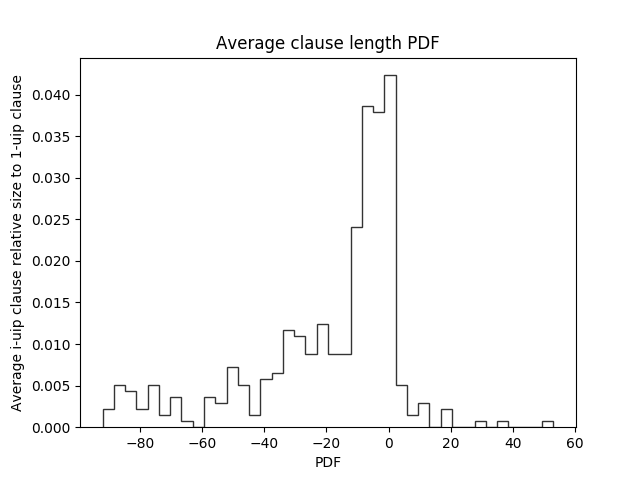
\includegraphics[width=0.8\textwidth,natwidth=610,natheight=642]{clause_length_PDF.png}
    \caption{Average clause (relative to 1-UIP clauses) size distribution. X axis indicates the relative size difference, and Y axis indicates the PDF.}
     \label{fig:len_pdf}
\end{figure}
\begin{figure} \label{fig:len_compare}
    \centering
    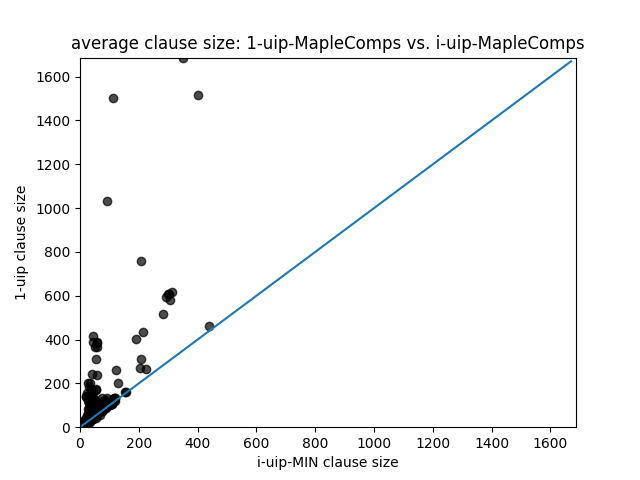
\includegraphics[width=0.8\textwidth,natwidth=610,natheight=642]{i-uip-sizes-compare.png}
    \caption{Average clause size comparison plot. Each point in the plot represents an benchmark instance. X and Y axis shows the clause length from $\IUIP$ and 1-UIP, respectively. Each green (red) dot represents an compared instance between $\MapleBase$ and $\MapleIUIMIN$ ($\IUIPPURE$).   }
    \label{fig:len_compare}
\end{figure}


$\IUIPMIN$ outperformed $\IUIPPURE$ in both PAR-2 score and clause size.  This results agrees with our observation in Fig.~\ref{fig:t2}: $\IUIPMIN$ attempted $\IUIP$ learning more frequently, and it is more likely to succeed. Remark that the success of $\IUIP$ learning is determined by the size of the learned i-UIP clause $\iUIPClause$, and the $\IUIP$ learning frequency is also indirectly controlled by $\IUIP$'s success rate from the previous restart interval. The results indicates  $\IUIPMIN$ shortened $\iUIPClause$'s size through further minimization of $\iUIPClause$ at non-unique implication decision level.



\begin{figure} 
\begin{center} 
\begin{tabular}{ | m{3.5cm} | m{5cm}| m{5cm} | } 
\hline
Solver & $\IUIP$ attempt rate & $\IUIP$ success rate  \\ 
\hline
$\MapleIUIPPURE$ & 16.1\% & 43.4\% \\ 
\hline
$\MapleIUIMIN$ & 28.8\% & 59.3\% \\ 
\hline
\end{tabular}
\end{center}
\caption{Compare $\IUIPPURE$ and $\IUIPMIN$ i-uip attempt rate and success rate. $\IUIPMIN$ scheme attempted $\IUIP$ more frequently, and it is more likely to successfully produce smaller $\iUIPClause$ clause .}
\label{fig:t2}
\end{figure}

A solver produce smaller clauses can construct smaller proofs. For UNSAT instances, we additionally measure their DRUP\cite{} proof checking time as well as the size of the optimized DRUP proof. We used DART-trim \cite{} with 5000 timeout to check and optimize DRUP proofs. 

Fig.~\ref{fig:t3} shows that the optimized proof construct by $\IUIPMIN$ and $\IUIPPURE$ are significantly smaller than 1-UIP proofs. The relative proof size reduction roughly correlates to the average clause size reduction. Fig.~\ref{fig:proof_compare} shows the absolute proof size comparison results. 

\begin{figure} 
\begin{center} 
\begin{tabular}{ | m{3.5cm} | m{5cm}| m{5cm} | } 
\hline
Solver & optimized proof size (MB) & relative reduction size  \\ 
\hline
$\MapleBase$ & 613.9 & 0  \\ 
\hline
$\MapleIUIPPURE$ & 487.2 & 6.90\% \\ 
\hline
$\MapleIUIMIN$ & 413.2 & 17.18\% \\ 
\hline
\end{tabular}
\end{center}
\caption{Optimized UNSAT proof comparison for 1-UIP $\IUIPPURE$ and $\IUIPMIN$. Optimized proof size measures the average absolute proof size in MB, and relative reduction size measures the average relative reduction for all UNSAT instances.}
\label{fig:t3}
\end{figure}

\begin{figure}
    \centering
    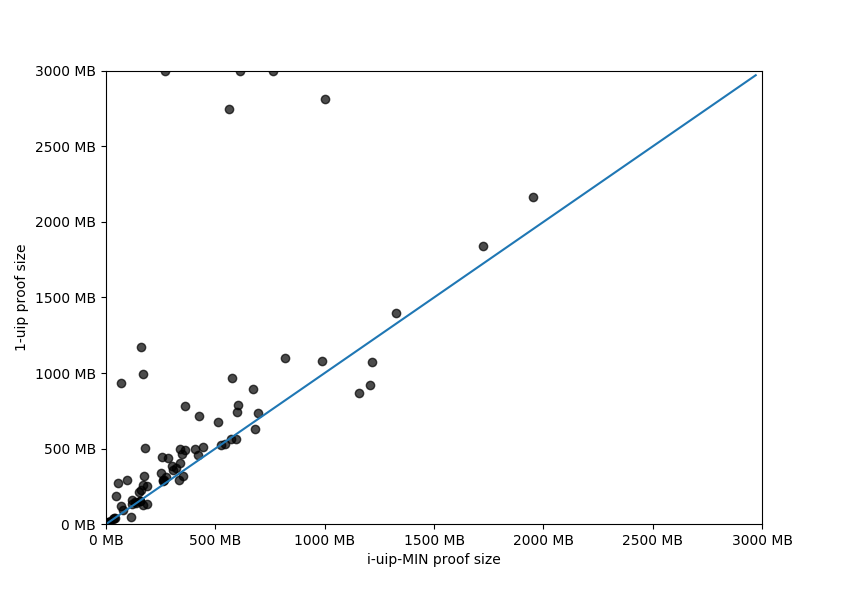
\includegraphics[width=0.8\textwidth,natwidth=610,natheight=642]{proof_size_compare.png}
    \caption{Average optimized proof size between 1-uip and $\IUIPMIN$.}
    \label{fig:proof_compare}
\end{figure}

\subsection{$\IUIP$ as a Practical Learning Scheme}
To evaluate $\IUIP$'s effectiveness as a clause learning scheme, we implement $\IUIPMIN$ on $\MapleBase$ with the extensions mentioned in section~\ref{sec:i-uip}. We evaluated four different configurations (i-UIP, i-UIP-Greedy, i-UIP-Inclusive, and i-UIP-Exclusive) of $\IUIP$ and 1-UIP learning on the SAT Race 2019 main track benchmark and report each configuration's solved instances, PAR-2 score and average clause size. 

Fig.~\ref{fig:t4} summarizes the result of the experiment. Learning scheme i-UIP-greedy solves the same amount of instance (226) as i-UIP with less PAR-2 score. The inclusive activity adjustment solves the most SAT instances (138) and the least UNSAT instances (87). The exclusive activity adjustment scheme produces the shortest average clause size, but solved the second least instances, one more instance than the baseline.  

\begin{figure} 
\begin{center}
\begin{tabular}{ | m{3.5cm} | m{4cm}| m{2cm} | m{2.75cm} |  } 
\hline
Solver & \# solved (SAT, UNSAT) & PAR-2 & Avg clause Size \\ 
\hline
1-UIP & 221 (132, 89)  & 5018.89 & 62.6  \\ 
\hline
i-UIP & \textbf{226} (135, \textbf{91}) & 4890.67 & 45.2 \\ 
\hline
i-UIP-greedy & \textbf{226} (135, \textbf{91})  & \textbf{4866.94} & 47.7 \\
\hline
i-UIP-active-Inclusive & 225 (\textbf{138}, 87) & 4958.49 & 52..12 \\
\hline
i-UIP-active-Exclusive & 223 (134, 89) & 5015.23 & \textbf{43.2} \\
\hline
\end{tabular}
\end{center}
\caption{Benchmark results of 1-UIP ($\MapleBase$), i-UIP($\IUIPMIN$), i-UIP-Greedy,
i-UIP-Inclusive, and i-UIP-Exclusive on SAT2019 race main track.}
\label{fig:t4}
\end{figure}


\nf{Inserted a table here, and graphs and analysis}


\subsection{$\IUIP$ on Modern SAT solvers}
To validate $\IUIP$ as a generalizable learning scheme on modern SAT solvers, we re-implement $\IUIP$ on $\MapleSeven$ \cite{},  $\MapleNine$ \cite{}($\MapleNineShort$) and $\expSAT$\cite{} ($\expSATShort$).  
The first two solvers are the winner of 2017 and 2019 SAT race, respectively.  $\expSATShort$ is a top ten solver from 2019 SAT race which uses random walk simulation to help branching. We chose $\expSATShort$ because 1) it is the best solver in the 2019 SAT Race without using chronological backtracking; 2) the random walk simulation branching heuristic allows our learning schemes to partially sidestep the problem of variable activity. For each solver, we compare the base 1-UIP learning scheme against $\IUIP$ learning and the top two $\IUIP$ variants, $\IUIPGreedy$ and $\IUIPActive$, on the SAT Race 2019 main track benchmark. We report solved instances, PAR-2 score and the average clause size.

\begin{figure} 
\begin{center}
\begin{tabular}{ | m{3.7cm} | m{4cm}| m{2cm} | m{2.75cm} |  } 
\hline
Solver & \# solved (SAT, UNSAT) & PAR-2 & Avg clause Size \\ 
\hline
$\MapleSeven$ & 232 (135, 97)  & 4755.96 & 61.9  \\ 
\hline
$\MapleSeven$-i-uip & \textbf{240} (\textbf{144}, 96) & \textbf{4601.25} & \textbf{36.97} \\ 
\hline
$\MapleSeven$-i-greedy & 237 (140, \textbf{97}) & 4678.434 & 43.62 \\ 
\hline
$\MapleSeven$-i-inclusive & 234 (137, 97) & 4718.03 & 37.96 \\ 
\hline
\hline
$\expSATShort$ & 237 (137, 100)  & 4628.96 & 63.19 \\
\hline
$\expSATShort$-i-uip & TBA & TBA & TBA \\ 
\hline
$\expSATShort$-i-greedy & 244 (143, \textbf{101}) & \textbf{4460.92} & 47.25 \\
\hline
$\expSATShort$-i-inclusive & \textbf{245} (\textbf{146}, 99) & 4475.76 & \textbf{45.33} \\
\hline
\hline
$\MapleNineShort$ & 243 (145, \textbf{98}) & 4450.24 & 61.00 \\
\hline
$\MapleNineShort$-i-uip & 244 (148, 96) & \textbf{4409.88} & \textbf{37.43} \\
\hline
$\MapleNineShort$-i-greedy & 243 (146, 97) & 4476.73 & 40.65 \\
\hline
$\MapleNineShort$-i-inclusive & \textbf{245} (\textbf{150}, 95) & 4425.99 & 37.60 \\
\hline
\end{tabular}
\end{center}
\caption{Benchmark results of 1-UIP, i-UIP($\IUIPMIN$), i-UIP-Greedy,
i-UIP-Inclusive on SAT2019 race main track.}
\label{fig:t5}
\end{figure}

Table~\ref{fig:t5} shows the benchmark result of $\IUIP$ configurations on different solvers. All three configurations of $\IUIP$ outperformed 1-UIP on $\MapleSeven$. i-UIP, i-UIP-Greedy and i-UIP-inclusive solved 8, 5 and 2 more instances, respectively, whiling producing smaller clauses.  The improvement of $\IUIP$ is more significant on $\MapleSeven$ than on $\MapleBase$ for both solved instances and clause size reduction. This may suggests that $\IUIP$ and the recent learnt clause minimization approach~\cite{} synergies well because: 1) i-UIP clauses are shorter with more common literals which allows vivification~\cite{} to prune literals more aggressively through unit propagation. 2) using $\IUIP$ instead of 1-UIP scheme to analyze conflicts during vivification could derive shorter clauses.

Similar to the observation on $\MapleSeven$, all three configurations of $\IUIP$ significantly outperformed 1-UIP on $\expSATShort$. i-UIP, i-UIP-Greedy and i-UIP-inclusive solved x, 7 and 8 more instances, respectively, while producing smaller clauses. We expect all three configurations of $\IUIP$ to solve the similar amount of instances with close PAR-2 scores because $\expSATShort$ allows the learning schemes to partially sidestep the activity problem. The learning adjustment for variable activities should have less impact on the solver's performance, and we observed the expected performance from the benchmark results. $\IUIP$ improved $\expSATShort$ the most across all compared solvers for both solved instances (+8) and PAR-2 score (-168), and this is might be due to the partially mitigation of the side-effect from variable activity.

$\IUIP$ learning schemes show moderate improvement on $\MapleNineShort$ as i-UIP, i-UIP-greedy and i-UIP-inclusive solved 1, 0 and 2 more instances, respectively, while producing smaller clauses. Our learning schemes didn't improve $\MapleNineShort$ significantly because the side-effects from chronological backtracking (CB). More specifically, We believe CB prevents decision levels from being compressed through the process of backtracking and re-asserting literals. Comparing to 1-uip clause, the shorter i-uip clauses can bring related literals tighter in a decision level, and consequently produces smaller decision levels with  backtracking. However, since CB discourages long distance backtracking, the effect of learning shorter clauses is shadowed until a full restart.  We believe we have observed an interesting interaction effect that shows the limitations of both CB and $\IUIP$ learning for future research.

